\clearpage
\section{Network Configuration and Access}
\label{sec:network}
\subsection{Three SSH Paths}
Figure~\ref{fig:laptop-robot-lan} shows the three ways Desktop reaches Pi. All addresses are fixed and all prefixes are /24. Path A is the Pi with only Wi-Fi connected. Paths B and C require the Pi Ethernet cable: plugged into an ASUS LAN port for B, and into the home router for C.

\begin{figure}[H]
\centering
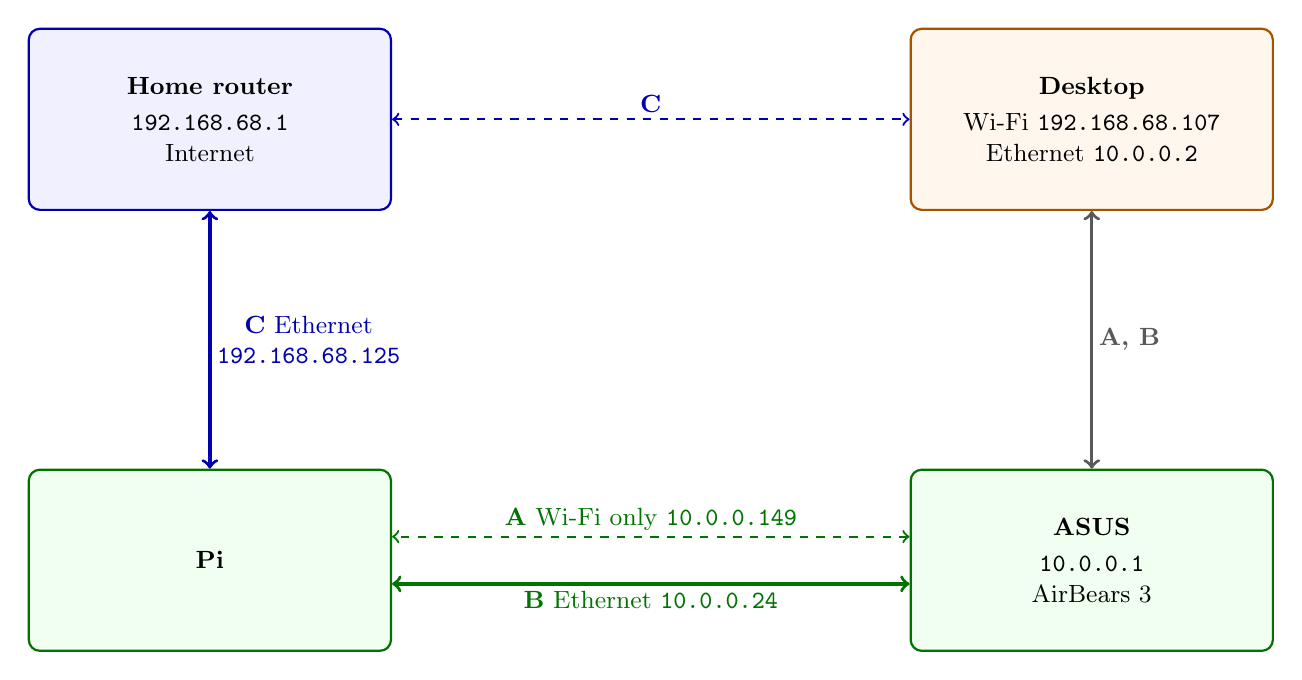
\begin{tikzpicture}[
    box/.style={draw,thick,rounded corners,align=center,inner sep=7pt,
        font=\small,minimum width=4.6cm,minimum height=2.3cm},
    home/.style={box,draw=blue!70!black,fill=blue!6},
    mac/.style={box,draw=orange!65!black,fill=orange!7},
    pi/.style={box,draw=green!45!black,fill=green!6},
    asus/.style={box,draw=green!45!black,fill=green!6},
    lab/.style={font=\small,align=center,fill=white,inner sep=2pt},
    eth/.style={<->,very thick},
    wifi/.style={<->,thick,dashed}
]
\node[home] (home) at (0,0) {%
    \textbf{Home router}\\[2pt]
    \texttt{192.168.68.1}\\
    Internet};
\node[mac] (mac) at (11.2,0) {%
    \textbf{Desktop}\\[2pt]
    Wi-Fi \texttt{192.168.68.107}\\
    Ethernet \texttt{10.0.0.2}};
\node[pi] (pi) at (0,-5.6) {\textbf{Pi}};
\node[asus] (asus) at (11.2,-5.6) {%
    \textbf{ASUS}\\[2pt]
    \texttt{10.0.0.1}\\
    AirBears 3};
\draw[wifi,blue!70!black] (home.east) -- node[lab,above] {\textbf{C}} (mac.west);
\draw[eth,black!65] (mac.south) -- node[lab,right] {\textbf{A, B}} (asus.north);
\draw[wifi,green!45!black] ([yshift=3mm]asus.west) --
    node[lab,above] {\textbf{A}\ Wi-Fi only\ \texttt{10.0.0.149}} ([yshift=3mm]pi.east);
\draw[eth,green!45!black] ([yshift=-3mm]asus.west) --
    node[lab,below] {\textbf{B}\ Ethernet\ \texttt{10.0.0.24}} ([yshift=-3mm]pi.east);
\draw[eth,blue!70!black] (home.south) --
    node[lab,right] {\textbf{C}\ Ethernet\\ \texttt{192.168.68.125}} (pi.north);
\end{tikzpicture}

\caption{SSH paths. The host name is pi2. A, Wi-Fi only: \texttt{ssh pi2} at \texttt{10.0.0.20}. B and C require the Ethernet cable. B: that cable to ASUS, \texttt{ssh pi2-asus-eth} at \texttt{10.0.0.120}. C: that cable to the home router, \texttt{ssh pi2-home-eth} at \texttt{192.168.68.220}. Desktop is \texttt{10.0.0.2} on A and B, and \texttt{192.168.68.107} on C. The login account is \texttt{pi}.}
\label{fig:laptop-robot-lan}
\end{figure}

\begin{table}[H]
\centering\small
\caption{Fixed SSH addresses.}
\label{tab:current-network}
\begin{tabular}{@{}lll@{}}
\toprule
Path & pi2 Address & Connection Details \\
\midrule
A & \texttt{10.0.0.20} & Wi-Fi only (to ASUS \texttt{AirBears 3}). Desktop on ASUS Ethernet \texttt{10.0.0.2}. \\
B & \texttt{10.0.0.120} & Ethernet cable to ASUS LAN port. Desktop on ASUS Ethernet \texttt{10.0.0.2}. \\
C & \texttt{192.168.68.220} & Ethernet cable to Home router. Desktop on Home Wi-Fi \texttt{192.168.68.107}. \\
\bottomrule
\end{tabular}
\end{table}

\subsection{Network Profiles and Routing}
The host name is \texttt{pi2} and the login user is \texttt{pi}. All subnet masks are \texttt{/24}.

\begin{itemize}
\item \textbf{Path A (\texttt{asus-robot})}: Wi-Fi connection to the ASUS router at \texttt{10.0.0.20/24} (gateway \texttt{10.0.0.1}).
\item \textbf{Path B (\texttt{asus-ethernet})}: Ethernet connection to the ASUS router at \texttt{10.0.0.120/24} (gateway \texttt{10.0.0.1}).
\item \textbf{Path C (\texttt{Wired connection 1})}: Ethernet connection to the home router at \texttt{192.168.68.220/24} (gateway and DNS \texttt{192.168.68.1}).
\end{itemize}

The script \texttt{select\_pi\_ethernet.sh} detects whether the Ethernet cable is connected to the ASUS router or the home router and activates \texttt{asus-ethernet} or \texttt{Wired connection 1} accordingly. The ASUS network operates isolated without requiring upstream Internet, while the home router provides direct Internet access.
